\section{Topología}

Si queremos conectar solo dos dispositivos, podemos conectarlos directamente con un enlace punto a punto. Cuando aumentemos el número de dispositivos, podemos usar un único elemento de red (conmutador o encaminador) de $N$ puertos para conectarlos. En el momento en el que tengamos más de $N$ dispositivos, necesitamos usar varios elementos de red que actúen de intermediarios, conectándolos entre ellos para aumentar el número de entradas disponibles de la red en la que conectar los dispositivos o \textit{nodos finales}.

Podemos describir la topología de una red como un grafo 
% $G=\langle V,A\rangle$ 
donde los vértices $V$ representan los elementos de red y $A$ los enlaces punto a punto entre ellos. Este grafo deberá ser fuertemente conexo para que todos los dispositivos tengan al menos un camino por el que llegar a cualquier otro dispositivo. El \textbf{número de saltos} es la cantidad de elementos de red por los que debe pasar un paquete para llegar a su destino, es decir, la longitud del camino que debe seguir.

Si usamos un grafo completo, tenemos una topología en la que cualquier nodo puede acceder a distancia mínima cualquier otro nodo, pero de mucho coste (más que un crossbar), necesitando encaminadores con tantos puertos como elementos en la red. Por ello, existen alternativas que consumen menos recursos, como las topologías en \textbf{bus} y en \textbf{anillo}, en las que se conectan los nodos finales mediante un solo cable central (figura \ref{fig:topology_busring}). En la topología en bus, la distancia máxima será de la longitud del bus, mientras que en la topología en anillo, esta distancia se reduce a la mitad porque el cable está cerrado, formando un ciclo.

\begin{figure}[p]
    \centering
    \begin{subfigure}[t]{.4\textwidth}
        \raisebox{6mm}{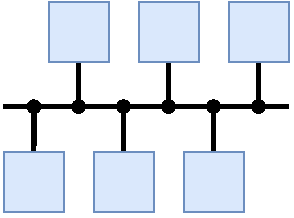
\includegraphics{images/diagrams/topology_bus.drawio.pdf}}
        \caption{Topología en bus.}
    \end{subfigure} %
    \hfill %
    \begin{subfigure}[t]{.4\textwidth}
        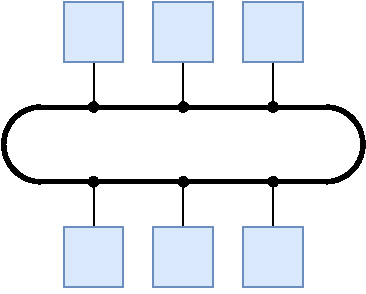
\includegraphics{images/diagrams/topology_ring.drawio.pdf}
        \caption{Topología en anillo.}
        \label{fig:topology_ring}
    \end{subfigure}
    \caption[Topologías de red en bus y en anillo.]{Topologías de red en bus y en anillo. Las conexiones de los nodos finales, simbolizadas con puntos negros, pueden ser tanto conexiones a un medio compartido como nodos intermedios.}
    \label{fig:topology_busring}
\end{figure}
\begin{figure}[p]
    \centering
    \begin{subfigure}[t]{.45\textwidth}
        \centering
        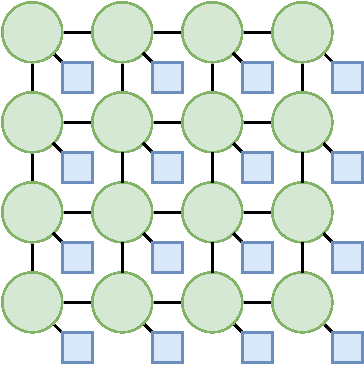
\includegraphics{images/diagrams/topology_mesh.drawio.pdf}
        \caption[Topología en malla bidimensional.]{Topología en malla bidimensional de 4x4. Cada nodo intermedio tiene conectado un nodo final y la distancia máxima es de 6 enlaces.}
        \label{fig:topology_mesh}
    \end{subfigure}\hfill
    \begin{subfigure}[t]{.5\textwidth}
        \centering
        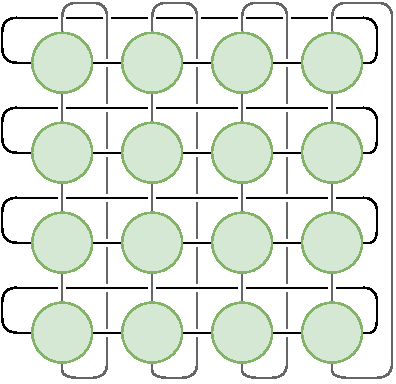
\includegraphics{images/diagrams/topology_thorus.drawio.pdf}
        \caption[Topología de toro bidimensional.]{Topología de toro bidimensional. Su distancia máxima es de 4 enlaces.}
        \label{fig:topology_thorus}
    \end{subfigure}
    \caption{Topologías en malla y toro.}
    \label{fig:topology_mesh_thorus}
\end{figure}

Aumentando el número de nodos intermedios, se pueden formar topologías más complejas. Por ejemplo, con una rejilla N-dimensional de aristas conectadas cada una de ellas con su adyacente, se forma una topología en \textbf{malla} (figura \ref{fig:topology_mesh}). La distancia máxima será la distancia Manhattan entre los nodos más lejanos (las esquinas opuestas), igual a la suma de la distancia de el número de vértices en los dos lados: $D = (l_1-1)+(l_2-1)$. Esta distancia máxima puede reducirse cerrando los extremos y formando un \textbf{toro}, acortándose a la suma de la división entera de los lados entre dos: $D = \lfloor l_1/2\rfloor + \lfloor l_2/2\rfloor$.

Según \cite{Duato03} y \cite{HenessyPattersonF}, dependiendo de como se conecten los nodos finales entre sí, podemos clasificar las redes de interconexión en las siguientes clases:
\begin{itemize}
    \item \textbf{Medio compartido}: El medio es compartido entre todos los dispositivos y se necesita un método de detección o evitación de colisiones. Los buses, anillos y las redes inalámbricas serían redes de medio compartido.
    \item \textbf{Medio conmutado}: Se establece dinámicamente una vía de comunicación entre la fuente y el destino.
    \begin{itemize}
        \item \textbf{Dinámicas/Indirectas}: Los nodos finales se conectan únicamente en los bordes de la red, lo que permite que el número de nodos sea menor al de conmutadores. Serían ejemplos de este tipo de redes los crossbars o las redes de interconexión multietapa (MINs).
        \item \textbf{Estáticas/Directas}: Cada encaminador está conectado directamente con un nodo emisor, no sólo en la periferia de la red, por lo que el número de encaminadores es igual al número de nodos, como en la topología en malla de la figura \ref{fig:topology_mesh}
    \end{itemize}
\end{itemize}

\begin{recuadronoc}
    Nuestra red es una \textbf{\textit{malla}} bidimensional de encaminadores. Aunque las mallas normalmente forman redes \textit{directas}, nosotros hemos usado encaminadores de 4 puertos, aprovechando los extremos de la malla para conectar los nodos finales. Por lo tanto, nuestra malla sería una red \textit{indirecta}.
\end{recuadronoc}

\subsection{Tipos de enlace}
En las redes de medio conmutado, llamamos enlace a cada uno de los canales que conectan directamente dos dispositivos.
Según el sentido de la transmisión, podemos distinguir los siguientes tipos:

\begin{itemize}
    \item \textbf{Símplex}: Conexión unidireccional entre los dos elementos. El emisor puede enviar datos al receptor, pero no recibirlos de este.
    \item \textbf{Full-Dúplex}: Conexión bidireccional simultánea, en la que los dos elementos conectados pueden hacer uso de la conexión paralelamente, transmitiendo y recibiendo información al mismo tiempo.
    \item \textbf{Half-dúplex}: Conexión bidireccional compartida, en la que si un elemento está transmitiendo, el enlace queda ocupado. La principal ventaja es que se necesitan la mitad de recursos que full-dúplex.
\end{itemize}

\begin{recuadronoc}
    En nuestra NoC nos hemos decantado por usar conexiones \textbf{full-dúplex} entre los nodos, pues las distancias entre ellos son tan cortas que el ahorro en cable sería insignificante, requiriendo implementar algún tipo de arbitraje en los enlaces para evitar colisiones cuando en un instante de tiempo los dos nodos quieran acceder al mismo.
\end{recuadronoc}
